\documentclass{article}
\usepackage{hyperref}
\usepackage{listings}
\usepackage{color}
\usepackage{xcolor}
\usepackage{geometry}
\usepackage{graphicx}
\usepackage{amsmath}
\usepackage{caption}
\usepackage{subcaption}
\usepackage{syntax}
\geometry{margin=1in}
\pdfminorversion=6

\newcommand\TODO[1]{\textcolor{red}{TODO: #1}}

\newcommand\header[2]{
    \begin{center}
        {\large
        UCSD CSE 291 (Differentiable Programming) Assignment #1: \\
        \vspace{0.3cm}
        \Large
        #2}
    \end{center}
}

\definecolor{dkgreen}{rgb}{0,0.6,0}
\definecolor{gray}{rgb}{0.5,0.5,0.5}
\definecolor{mauve}{rgb}{0.58,0,0.82}
\lstset{frame=tb,
        aboveskip=3mm,
        belowskip=3mm,
        showstringspaces=false,
        columns=flexible,
        basicstyle={\small\ttfamily},
        numbers=none,
        numberstyle=\tiny\color{gray},
        keywordstyle=\color{blue},
        commentstyle=\color{dkgreen},
        stringstyle=\color{mauve},
        breaklines=true,
        breakatwhitespace=true,
        tabsize=2
}

\hypersetup{colorlinks=true}


\begin{document}

\header{3}{Handling control flow and function calls}

Now we are going to extend our previous implementations of forward and reverse modes to handle: if/else statements, general function calls, and while loops. We will dive into each case immediately! As usual, use \lstinline{hw_tests/hw3/test.py} to test your implementation.

\section{Handling if/else statements}

Handling if/else statements in both forward and reverse modes are as simple as passing down the then and else statements and process them independently in the \lstinline{mutate_ifelse} method. 

\paragraph{Forward mode.} For example, the following code
\begin{lstlisting}[language=Python]
def ifelse(x : In[float], y : In[float]) -> float:
    ret : float
    if y > 0.0:
        ret = 5.0 * x
    else:
        ret = 2.0 * x
    return ret

fwd_ifelse = fwd_diff(ifelse)
\end{lstlisting}
would be transformed into something like:
\begin{lstlisting}[language=Python]
def fwd_ifelse(x : In[_dfloat], y : In[_dfloat]):
    ret : _dfloat
    if y.val > 0.0:
        ret = make__dfloat(5.0 * x.val, 0.0 * x.val + 5.0 * x.dval
    else:
        ret = make__dfloat(2.0 * x.val, 0.0 * x.val + 2.0 * x.dval
    return make__dfloat(ret.val, ret.dval)
\end{lstlisting}
(Note that we keep the condition unchanged, we will discuss in the class about methods that do handle the conditions.)

\lstinline{test_ifelse_fwd} tests for this.

\paragraph{Reverse mode.} Reverse mode works similarly: we copy the if else structure in both the forward and reverse passes, but run statements backwards in the reverse pass. The function above would be transformed into something like:
\begin{lstlisting}[language=Python]
def rev_ifelse(x : In[float], _dx : Out[float], y : In[float], _dy : Out[float], _dreturn : In[float]):
    # Forward pass
    _t_float : Array[float, 2]
    _stack_ptr_float = 0
    ret : float
    _dret : float
    if y > 0.0:
        _t_float[_stack_ptr_float] = ret
        _stack_ptr_float = _stack_ptr_float + 1
        ret = 5.0 * x
    else:
        _t_float[_stack_ptr_float] = ret
        _stack_ptr_float = _stack_ptr_float + 1
        ret = 2.0 * x
    # Reverse pass
    _adj_0 : float
    _adj_1 : float
    _dret = _dret + _dreturn;
    if y > 0.0:
        _stack_ptr_float = _stack_ptr_float - 1
        ret = _t_float[_stack_ptr_float]
        _adj_0 = 5.0 * _dret
        _dret = 0.0
        _dx = _dx + _adj_0
    else:
        _stack_ptr_float = _stack_ptr_float - 1
        ret = _t_float[_stack_ptr_float]
        _adj_1 = 2.0 * _dret
        _dret = 0.0
        _dx = _dx + _adj_1
\end{lstlisting}

\lstinline{test_ifelse_rev} tests for this.

We additionally have two more tests for reverse mode: \lstinline{test_ifelse_side_effects_rev} and \lstinline{test_nested_ifelse_rev}. You shouldn't need to do something special to pass these two tests.

\section{Handling function calls.}

\paragraph{Forward mode.} You most likely only need to modify \lstinline{mutate_call(self, node)} to handle the case when \lstinline{node.id} is not one of the intrinsic functions. Inside it, you will need to turn the arguments into their \lstinline{_d} counterparts in order to call the function. For reference, the following code:
\begin{lstlisting}[language=Python]
def foo(x : In[float], y : In[float]) -> float:
    return x * x * y + y * y

def func_call(x : In[float], y : In[float]) -> float:
    z : float = foo(x, y)
    return 2 * z

fwd_func_call = fwd_diff(func_call)
\end{lstlisting}
will be transformed to
\begin{lstlisting}[language=Python]
def _d_fwd_foo(x : In[_dfloat], y : In[_dfloat]) -> _dfloat:
    return make__dfloat(x.val * x.val * y.val + y.val * y.val,
    x.dval * x.val + x.val * x.dval * y.val + x.val * x.val * y.dval + y.dval * y.val + y.val * y.dval)

def fwd_func_call(In[_dfloat] x, In[_dfloat] y) -> _dfloat:
    z : _dfloat = make__dfloat(\
        _d_fwd_foo(make__dfloat(x.val, x.dval), make__dfloat(y.val, y.dval)).val,
        _d_fwd_foo(make__dfloat(x.val, x.dval), make__dfloat(y.val, y.dval)).dval)
    return make__dfloat(2 * z.val, 0.0 * z.val + int2float(2) * (z.dval))
\end{lstlisting}
Use the \lstinline{func_to_fwd} argument in the \lstinline{forward_diff} function to map function names to their forward differentiation counterpart.

Notice that in my implementation, \lstinline{_d_fwd_foo} is called twice. This does not affect the correctness since \lstinline{_d_fwd_foo} does not have side effects (partly why we restricted function calls with outputs arguments to only be in \lstinline{CallStmt}). My hope is that the downstream compiler would recognize that the two calls give the same results and optimize this in a common subexpression elimination pass. Otherwise, it should be possible to optimize this ourselves (e.g., using the \lstinline{CallNormalizeMutator} we will introduce later). This optimization is not required in this homework.

The next test is \lstinline{test_chained_calls_fwd}. This test asks you to differentiate function compositions like \lstinline{f(g(h(x)))}. You should not need to do anything extra to pass this test.

The next test is \lstinline{test_call_stmt_fwd}:
\begin{lstlisting}[language=Python]
def foo(x : In[float], y : Out[float]):
    y = x * x + x

def call_stmt(x : In[float]) -> float:
    y : float
    foo(x, y)
    return 2 * y

fwd_call_stmt = fwd_diff(call_stmt)
\end{lstlisting}
If you implement the previous parts like me, you might generate a function call like:
\begin{lstlisting}[language=Python]
# def _d_fwd_foo(x : In[_dfloat], y : Out[_dfloat]):
_d_fwd_foo(make__dfloat(x.val,x.dval), make__dfloat(y.val,y.dval))
\end{lstlisting}
However, since the second argument \lstinline{y} is an output argument, this is not a legal loma code. My solution is: whenever we encounter an output argument in a function call in forward mode, we just switch to the original argument. In the case above my implementation would output the call statement: \lstinline{_d_fwd_foo(make__dfloat(x.val,x.dval), y)}.

\paragraph{Reverse mode} Handling function calls in reverse mode is slightly more annoying. Firstly, we need to modify \lstinline{mutate_call} to handle functions outside of the built-in ones. For example, consider the following \lstinline{CallStmt}:
\begin{lstlisting}[language=Python]
# def foo(x : In[float], y : In[float], z : Out[float])
foo(x, y, z)
\end{lstlisting}
It should be transformed into
\begin{lstlisting}[language=Python]
# def _d_foo(x : In[float], _dx : Out[float], y : In[float], _dy : Out[float], _dz : In[float])
d_foo(x, _dx, y, _dy, _dz)
\end{lstlisting}
Notice that for each input argument (\lstinline{x} and \lstinline{y} in this case), we append another output argument to receive the derivatives. For each output argument, we turn them into an input argument that receives the adjoint.
(As in forward mode, use the argument \lstinline{func_to_rev} to map function names to their reverse mode counterpart.)

However, if you do this naively, you will run into some problems with a function call like this:
\begin{lstlisting}[language=Python]
# bar(a : In[float], b : In[float], c : Out[float])
bar(2 * x, y + x, z) # 2 * x and y + x are inputs, z is output
\end{lstlisting}
We do not have specific variables for storing \lstinline{2 * x} and \lstinline{y + x}'s adjoint. 

Furthermore, side effects are even more annoying when differentiating function calls. Consider the following function call:
\begin{lstlisting}[language=Python]
# foobar(a : In[Array[float]])
a[5] = foobar(a)
\end{lstlisting}
Using our previous way to differentiate this function call, we will need to store the derivatives of \lstinline{a} into an entire temporary array, then accumulate to the final derivative buffer -- this is prohibitively slow (and can change the complexity of reverse mode!). 

Our solution to this is to factor out the expressions inside the function arguments, until they can be used as a left hand side in an assign statement. For the \lstinline{bar} example above, we first rewrite the original call statement as:
\begin{lstlisting}[language=Python]
_x : float = 2 * x
_y : float = y + x
bar(_x, _y, z)
\end{lstlisting}
Then we can transform \lstinline{bar(_x, _y, z)} into something like \lstinline{d_bar(_x, __dx, _y, __dy, _dz)}.

For the \lstinline{foobar} function, we perform the following rewrite:
\begin{lstlisting}[language=Python]
# foobar(a : In[Array[float]])
t : float
t = foobar(a)
a[5] = t
\end{lstlisting}
Now, there is no clash of the use of \lstinline{a} in the assign statement and we can safely differentiate.

We have provided the code for doing the rewrite for you already: look at \lstinline{CallNormalizeMutator} in \lstinline{reverse_diff.py}. You can apply it at the beginning of \lstinline{mutate_function_def}.

Finally, we still have to deal with the variables overwrite with function calls. You need to do the same thing as we did with the assign statements but for \lstinline{CallStmt} (we disallowed function calls with outputs outside of call statement to simplify this part). For reference, the following code in \lstinline{test_call_stmt_side_effect}:
\begin{lstlisting}[language=Python]
def foo(x : In[float], y : Out[float]):
    y = x * x + x

def call_stmt_side_effects(x : In[float]) -> float:
    y : float = 10.0
    z : float = y * x
    foo(x, y)
    return 2.0 * y + z

rev_call_stmt_side_effects = rev_diff(call_stmt_side_effects)
\end{lstlisting}
Would be transformed into something like
\begin{lstlisting}[language=Python]
def rev_call_stmt_side_effects(x : In[float], _dx : Out[float], _dreturn : In[float]):
    _t_float : Array[float, 1]
    _stack_ptr_float : int
    y : float = 10.0
    _dy : float
    z : float = y * x
    _dz : float
    _t_float[_stack_ptr_float] = y
    _stack_ptr_float = _stack_ptr_float + 1
    foo(x, y)
    _dy = _dy + 2.0 * _dreturn
    _dz = _dz + _dreturn
    _stack_ptr_float = _stack_ptr_float - 1
    y = _t_float_[_stack_ptr_float]
    _d_rev_foo(x, _dx, _dy)
    _dy = 0.0
    _dy = _dy + x * _dz
    _dx = _dx + y * _dz
\end{lstlisting}

The tests for call expressions and statements in reverse mode are: \lstinline{test_func_call_rev}, \lstinline{test_func_call_rev2}, \lstinline{test_func_call_assign_rev}, \lstinline{test_call_array_rev}, \lstinline{test_call_stmt_rev}, \lstinline{test_call_stmt2_rev}, \lstinline{test_call_stmt_side_effects}, \lstinline{test_call_stmt_side_effects2}, \lstinline{test_call_stmt_array_rev}, and \lstinline{test_chained_calls_rev}.

\section{Handling while loops.}

\paragraph{Forward mode.} Handling while loops in forward mode is pretty much the same as in the if/else statements: we can simply pass in the body of the loop, and do nothing to the while condition. You will implement the \lstinline{mutate_while} method for this.

For reference, the following code:
\begin{lstlisting}[language=Python]
def while_loop(x : In[float], n : In[int]) -> float:
    i : int = 0
    z : float = x
    while (i < n, max_iter := 10):
        z = sin(z)
        i = i + 1
    return z

fwd_while_loop = fwd_diff(while_loop)
\end{lstlisting}
will be transformed into something like:
\begin{lstlisting}[language=Python]
_def fwd_while_loop(x : In[_dfloat], n : In[int]) -> _dfloat:
    i : int i = 0
    z : _dfloat = make__dfloat(x.val, x.dval)
    while (i < n, max_iter := 10):
        z = make__dfloat(sin(z.val), cos(z.val) * z.dval)
        i = i + 1
    return make__dfloat(z.val, z.dval)
\end{lstlisting}

\lstinline{test_while_loop_fwd} tests for differentiating while loops in forward mode.

\paragraph{Reverse mode.} To handle reverse mode, we will need to run the while loop backwards. Consider a generic while condition:
\begin{lstlisting}[language=Python]
cond : int = #...
while (cond, max_iter := 50):
    # ...
\end{lstlisting}
How do we run this backwards in the reverse pass? A general solution is to add a loop counter in the forward pass:
\begin{lstlisting}[language=Python]
# Forward pass
cond : int = #...
_loop_counter : int = 0
while (cond, max_iter := 50):
    # ...
    _loop_counter = _loop_counter + 1

# Reverse pass
while (_loop_counter > 0, max_iter := 50):
    # ...
    _loop_counter = _loop_counter - 1
\end{lstlisting}
However, this simple solution will not directly work for nested loop. Consider the following transformed code:
\begin{lstlisting}[language=Python]
# Forward pass
cond0 : int = #...
cond1 : int = #...
_loop_counter_0 : int = 0
_loop_counter_1 : int = 0
while (cond0, max_iter := 50):
    # ...
    while (cond1, max_iter := 60):
        # ...
        _loop_counter_1 = _loop_counter1 + 1
    _loop_counter0 = _loop_counter0 + 1

# Reverse pass
_loop_counter_1_copy : int = #...
while (_loop_counter_0 > 0, max_iter := 50):
    # ...
    _loop_counter_1_copy = _loop_counter_1
    while (_loop_counter_1_copy > 0, max_iter := 60):
        # ...
        _loop_counter_1_copy = _loop_counter_1_copy - 1
    _loop_counter_0 = _loop_counter_0 - 1
\end{lstlisting}
This is incorrect, because there is no guarantee that the inner loop would have the same \lstinline{_loop_counter_1} for each outer loop iteration.

Instead, the following is the correct transformation:
\begin{lstlisting}[language=Python]
# Forward pass
cond0 : int = #...
cond1 : int = #...
_loop_counter_0 : int = 0
_loop_counter_1 : Array[int, 50]
_loop_counter_1_ptr : int = 0
_loop_counter_1_tmp : int
while (cond0, max_iter := 50):
    # ...
    _loop_counter_1_tmp = 0
    while (cond1, max_iter := 60):
        # ...
        _loop_counter_1_tmp = _loop_counter_1_tmp + 1
    # push the loop counter to a stack
    _loop_counter_1[_loop_counter_1_ptr] = _loop_counter_1_tmp
    _loop_counter_1_ptr = _loop_counter_1_ptr + 1
    _loop_counter0 = _loop_counter0 + 1

# Reverse pass
while (_loop_counter_0 > 0, max_iter := 50):
    # ...
    # pop the loop counter from a stack
    _loop_counter_1_ptr = _loop_counter_1_ptr - 1
    _loop_counter_1_tmp = _loop_counter_1[_loop_counter_1_ptr]
    while (_loop_counter_1_tmp > 0, max_iter := 60):
        # ...
        _loop_counter_1_tmp = _loop_counter_1_tmp - 1
    _loop_counter_0 = _loop_counter_0 - 1
\end{lstlisting}
Notice that we push the inner loop counter to a stack in the forward pass, and then pop it back from the stack in the reverse pass. We allocate a fixed size array for the loop counter. 

Next, we need to deal with variable rewrites. Consider the following loop:
\begin{lstlisting}[language=Python]
def while_loop(x : In[float], n : In[int]) -> float:
    i : int = 0
    z : float = x
    while (i < n, max_iter := 10):
        z = sin(z)
        i = i + 1
    return z

rev_while_loop = rev_diff(while_loop)
\end{lstlisting}
Since \lstinline{z} is overwritten every iteration, we need to store its value per iteration in a stack:
\begin{lstlisting}[language=Python]
def rev_while_loop(x : In[float], _dx : Out[float], n : In[int], _dn : Out[int], _dreturn : In[float]):
    _t_float : Array[float, 10]
    _stack_ptr_float : int
    _t_int_ : Array[int, 10]
    _stack_ptr_int : int
    _loop_var_0 : int
    i : int = 0
    z : float = x;
    _dz : float
    _loop_var_0 = 0
    while (i < n, max_iter := 10):
        _t_float[_stack_ptr_float] = z
        _stack_ptr_float = _stack_ptr_float + 1
        z = sin(z)
        _t_int[_stack_ptr_int] = i
        _stack_ptr_int = _stack_ptr_int + 1
        i = i + 1
        _loop_var_0 = _loop_var_0 + 1
    _adj_0 : float
    _dz = _dz + _dreturn
    while (_loop_var_0 > 0, max_iter := 10):
        _stack_ptr_float = _stack_ptr_float - 1
        z = _t_float[_stack_ptr_float]
        _adj_0 = cos(z) * _dz
        _dz = 0.0
        _dz = _dz + _adj_0
        _loop_var_0 = _loop_var_0 - 1
    _dx = _dx + _dz
\end{lstlisting}
If there are nested loops, then we estimate the size of the arrays by multiplying the \lstinline{max_iter} from all parent loops the assign/call statements are in.

\lstinline{test_while_loop_rev}, \lstinline{test_nested_while_loop_rev}, and \lstinline{test_three_level_while_loop_rev} test for differentiating while loops in reverse mode.

\section{Parallelism}
Finally, we will handle SIMD code that can create race conditions during differentiation. Consider the following code:
\begin{lstlisting}[language=python]
@simd
def parallel_copy(x : In[float],
                  z : Out[Array[float]]):
    i : int = thread_id()
    z[i] = x

rev_parallel_copy = rev_diff(parallel_copy)
\end{lstlisting}
The primal code is perfectly race condition free and will copy the input \lstinline{x} to the entries of output array \lstinline{z}.

If done naively, reverse mode would produce something like:
\begin{lstlisting}[language=python]
@simd
def rev_parallel_copy(x : In[float],
                      _dx : Out[float],
                      z : In[Array[float]]):
    i : int = thread_id()
    _dx = _dx + z[i] # race condition!
\end{lstlisting}
We are adding to a scalar buffer \lstinline{_dx} simultaneously from many threads, and this is in general not going to produce correct results. In fact, the ISPC backend compiler would straight out fail to compile because they do not allow directly storing thread varying values to a global buffer.

Therefore, we need to use \lstinline{atomic_add} instead:
\begin{lstlisting}[language=python]
@simd
def rev_parallel_copy(x : In[float],
                      _dx : Out[float],
                      z : In[Array[float]]):
    i : int = thread_id()
    atomic_add(_dx, z[i])
\end{lstlisting}

To implement this, you simply need to turn the previous adjoint accumulation code into \lstinline{atomic_add} I will let you figure out which one to turn. Note that we disallow reading from an output buffer and writing to an input buffer (\lstinline{atomic_add} is the only exception), this significantly simplifies a lot of the nasty corner cases.

We will only test on the ISPC backend. You shouldn't need to do anything different for the OpenCL backend though. We have three tests for the parallel automatic differentiation: \lstinline{test_parallel_copy}, \lstinline{test_parallel_add}, and \lstinline{test_parallel_reduce}.

\section{More examples}
Now that our compiler starts to support more features, we can do pretty crazy stuff. As usual, the examples below are not graded. You might need to modify your code a bit to run these examples.

\begin{figure}
\centering
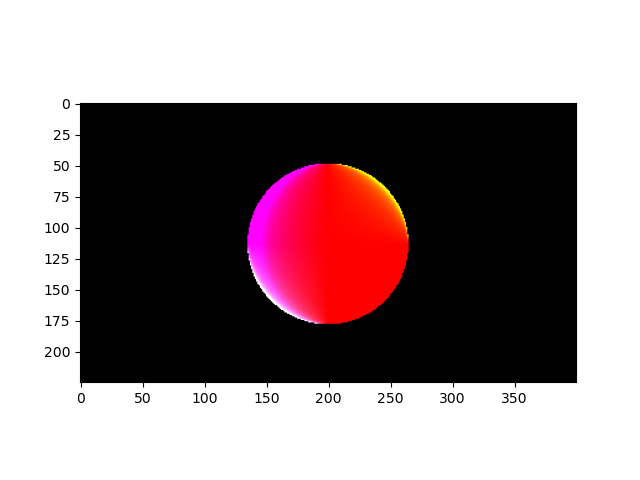
\includegraphics[width=0.8\linewidth]{imgs/diff_raytrace.png}
\vspace{-20pt}
\caption{Loma is used to compute the derivatives of normal with respect to camera position moving towards right.}
\label{fig:diff_raytrace}
\end{figure}

\subsection{Differentiable ray tracing}
Returning to our example in Homework 0, we can now compute derivatives inside our ray tracer. This can be useful for many things, including computer vision, and advanced rendering features. Figure~\ref{fig:diff_raytrace} shows an example where we compute the derivatives of the normal of the sphere, with respect to the camera position moving right. See \lstinline{examples/diff_raytrace_host} for the code.

\begin{figure}
\centering
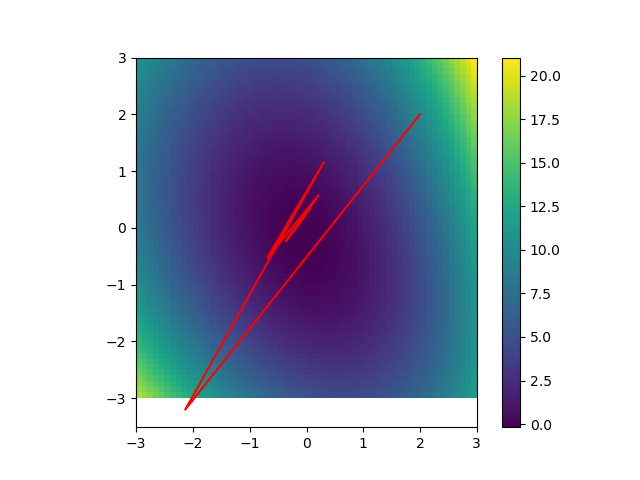
\includegraphics[width=0.8\linewidth]{imgs/optimize-newton.png}
\vspace{-20pt}
\caption{Revisiting the 2D optimization in Homework 1 using Newton's method.}
\label{fig:newton}
\end{figure}

\subsection{Second-order optimization}
Again, returning to our example in Homework 1, we can now compute second order derivatives of our 2D function and apply Newton's method for the optimization. We apply reverse mode on top of forward mode to compute the Hessian here:
\begin{lstlisting}[language=Python]
def grad_third_order_poly(x : In[float], y : In[float], gx : Out[float], gy : Out[float]):
    d_x : Diff[float]
    d_x.val = x
    d_x.dval = 1.0
    d_y : Diff[float]
    d_y.val = y
    d_y.dval = 0.0

    ret_x : Diff[float] = fwd_third_order_poly(d_x, d_y)
    gx = ret_x.dval
    d_x.dval = 0.0
    d_y.dval = 1.0
    ret_y : Diff[float] = fwd_third_order_poly(d_x, d_y)
    gy = ret_y.dval

rev_grad_poly = rev_diff(grad_third_order_poly)

def hess_third_order_poly(x : In[float], y : In[float],
                          hxx : Out[float], hxy : Out[float], hyy : Out[float]):
    rev_grad_poly(x, hxx, y, hxy, 1.0, 0.0)
    rev_grad_poly(x, hxy, y, hyy, 0.0, 1.0)
\end{lstlisting}
See \lstinline{examples/optimize_poly_hess.py} for the full code.

Figure~\ref{fig:newton} shows the optimization trajectory. With Newton's method, the optimization can take significantly larger step sizes and converges much faster than gradient descent.

\subsection{Mass spring model revisited}
We now revisit our mass spring model in Homework 2. I refactored the \lstinline{hamiltonian} function in the code so now it supports varying number of mass spring nodes:
\begin{lstlisting}[language=Python]
def square(x : In[float]) -> float:
    return x * x

def hamiltonian(q : In[Array[float]], p : In[Array[float]], c : In[MassSpringConfig]) -> float:
    K : float
    i : int = 0
    while (i < 2 * c.n, max_iter := 1000):
        K = K + 0.5 * p[i] * p[i] / c.mass
        i = i + 1

    U : float
    # mass spring potential
    tmp : float
    i = 0
    while (i < c.n - 1, max_iter := 1000):
        tmp = sqrt(square(q[2 * i] - q[2 * i + 2]) + square(q[2 * i + 1] - q[2 * i + 3])) - c.length
        U = U + 0.5 * c.k * tmp * tmp
        i = i + 1

    # gravity potential
    i = 0
    while (i < c.n, max_iter := 1000):
        U = U + c.mass * c.g * q[2 * i + 1]
        i = i + 1

    return K + U
\end{lstlisting}
See \lstinline{examples/mass_spring_rev_loop.py} for the full code. In \lstinline{examples/mass_spring_rev_loop.mp4}, we show an animation of a mass spring system with 40 nodes.

\end{document}
